%yright 2007, 2008, 2009 Elsevier Ltd
%% 
%% This file is part of the 'Elsarticle Bundle'.
%% ---------------------------------------------
%% 
%% It may be distributed under the conditions of the LaTeX Project Public
%% License, either version 1.2 of this license or (at your option) any
%% later version.  The latest version of this license is in
%%    http://www.latex-project.org/lppl.txt
%% and version 1.2 or later is part of all distributions of LaTeX
%% version 1999/12/01 or later.
%% 
%% The list of all files belonging to the 'Elsarticle Bundle' is
%% given in the file `manifest.txt'.
%% 

%% Template article for Elsevier's document class `elsarticle'
%% with numbered style bibliographic references
%% SP 2008/03/01

% \documentclass[preprint,11pt]{elsarticle}
\documentclass[final,1p,11pt]{elsarticle}

%\documentclass[final,1p,times]{elsarticle}


%% Use the option review to obtain double line spacing
%%\documentclass[authoryear,preprint,review,12pt]{elsarticle}

%% Use the options 1p,twocolumn; 3p; 3p,twocolumn; 5p; or 5p,twocolumn
%% for a journal layout:
%% \documentclass[final,1p,times]{elsarticle}
%% \documentclass[final,1p,times,twocolumn]{elsarticle}
%% \documentclass[final,3p,times]{elsarticle}
%% \documentclass[final,3p,times,twocolumn]{elsarticle}
%% \documentclass[final,5p,times]{elsarticle}
%% \documentclass[final,5p,times,twocolumn]{elsarticle}

%%% For including figures, graphicx.sty has been loaded in
%% elsarticle.cls. If you prefer to use the old commands
%% please give \usepackage{epsfig}


\usepackage{epsfig}
%\usepackage{cite}
%\usepackage{mcite}
\usepackage{array,tabularx,epsfig,mathrsfs,graphicx,rotating}
\usepackage{ifthen}
\usepackage{amsfonts}
\usepackage{ragged2e}
\PassOptionsToPackage{hyphens}{url}
\usepackage[hyphens]{url}
\usepackage{hyperref}
\usepackage{listings}
\usepackage{subfigure}
\usepackage{epstopdf}
% Custom colors
\usepackage{color}
\usepackage{float}

% to cross text
\usepackage[normalem]{ulem} % either use this (simple) or
\usepackage{soul} % use this (many fancier options)


\hypersetup{
  colorlinks=true,
  linkcolor=blue,
  citecolor=blue,
  urlcolor=blue
}




\graphicspath{{figs/}}


\pdfinfo{
   /Author (Chekanov/Demarteau)
   /Title  (Conceptual Design Studies for a CEPC Detector)
   /CreationDate (D:20160102195600)
   /Subject (PDFLaTeX)
   /Keywords (PDF;LaTeX)
}


\textheight=22cm
\textwidth=14.5cm

\newcommand{\beq}{\begin{equation}}
\newcommand{\eeq}{\end{equation}}
\newcommand{\la}{\langle}
\newcommand{\promc}{{\sc ProMC}}
\newcommand{\ra}{\rangle}
\newcommand{\eps}{\epsilon}
\newcommand{\ud}{\mathrm{d}}
\newcommand{\Ec}{\mathcal{E}}
\newcommand{\Fc}{\mathcal{F}}
\newcommand{\Za}{\mathrm{Z_1}}
\newcommand{\Zb}{\mathrm{Z_2}}
\newcommand{\Zn}{\mathrm{Z_n}}
\newcommand{\F}{\mathrm{F}}

\chardef\til=126
\newcommand{\mev}{{\,\mathrm{MeV}}}
\newcommand{\gev}{{\,\mathrm{GeV}}}
\newcommand{\tev}{{\,\mathrm{TeV}}}
\newcommand{\GEANTfour} {\textsc{geant4}}
\journal{XXX-XXX}



\begin{document}

\section{Studies of signal and background separation using Mann-Whitney U test}
%In this section, we study different jet substructure variables and compare their ability to separate the signal and the background for different detector sizes using Mann-Whitney U test.\\

%In the Mann Whitney U test by definition, if U value is closed to 0.5, it means two distributions have similar compositions, and we can't distinguish them very well. On the other hand, if U value of two distributions are closed to 0, it means both distributions' compositions are much different from each other. For another point of view, if U value is closed to 0.5, separation power of certain variable is bad, instead, if U value is closed to 0, separation power is great.\\

%Figure 6 shows the representative samples of the distributions about the U value for $\tau_{21}$,$\tau_{32}$ in different detector sizes. In $\tau_{21}$, separation power is improved when detector size is smaller, but in $\tau_{32}$, the smallest detector sizes isn't the best one to separate signal and background.\\

%In Figure 7, it shows the summary plots about the clustering in Mann Whitney U test in three different variables. In $\tau_{21}$, 5TeV has better separation power when detector sizes are getting smaller, but when energy higher than that, there is no improvement in smaller detector. In $\tau_{32}$, the case is similar to  $\tau_{21}$. Even worse, at some collision energies, bigger detector sizes have better separation power than smaller detector sizes. In $c_2^{(1)}$, all separation power aren't improved by detector sizes.  In summary, $c_2^{(1)}$ is the best parameter, because all values are smaller than other parameters compare with the same energy collision, and its separation power don't have the significant improvement in higher energy collision.\\

%In Figure 8 , it shows the summary plots about the rawhit cut at 0.5GeV in Mann Whitney U test in three different variables. In $\tau_{21}$, 5TeV and 10TeV have better separation power in smaller separation power, but when energy higher than that, it won't improve.  In $\tau_{32}$, all separation power aren't improved by detector sizes. In $c_2^{(1)}$, we can see in 5,10,20TeV, separation power will be improved slightly, but at 40TeV, it won't improve. In summary, $c_2^{(1)}$ has the highest power separation at highest collision energy.\\

In this section, we study different jet substructure variables and compare their ability to separate the signal and background for different detector cell sizes using the Mann-Whitney U test.\\

By the definition of the Mann-Whitney U test, if the value of U is close to 0.5, it means that the signal and background distributions have almost identical shapes, i.e. the separation power of the variable is bad. On the other hand, if the U value is close to 0, it means that the distributions of the signal and the background are very different from each other and the separation power of the variable is great.\\
 
Figure \textcolor{blue}{6} shows the representative sample of the distributions for $\tau_{21}$,$\tau_{32}$, in different detector sizes with their corresponding U value. In $\tau_{21}$, the separation power is better when the detector size is smaller. However, the separation power of tau32 does not improve when the detector size gets smaller.\\

Figure \textcolor{blue}{7} shows the summary plots of the clustering in Mann-Whitney U test for the three different variables.  In $\tau_{21}$, 5 TeV has the better separation power when the detector size is smaller. However, there is not much improvement in higher energy collisions. In $\tau_{32}$, 5 TeV has also better separation power on smaller detector size but higher energy collisions seem to have better separation power when the detector size is bigger. The $c_2^{(1)}$ does not seem to have any significant improvement in its separation power as the detector size gets smaller for all energy collision. Nevertheless, the U values of the $c_2^{(1)}$ are better than the$\tau_{21}$ and $\tau_{32}$. In conclusion, the $c_2^{(1)}$ variable is the best parameter as its separation power is better than the other variable and does not have a significant improvement in higher energy collision.\\

Figure \textcolor{blue}{8} shows the summary plots of the rawhit cut at 0.5 GeV in Mann Whitney U test for the three different variables. In $\tau_{21}$, 5 and 10 TeV have better separation power on smaller detector sizes. However, there is no significant improvement in the separation power of higher energy collisions. The $\tau_{32}$ does not have any significant improvement in its separation power as the detector size gets smaller for all energy collision. Lastly, there is a slight improvement in separation power for 5, 10, and 20 TeV energy collision in $c_2^{(1)}$. At 40 TeV, no significant improvement is observed. In conclusion, the $c_2^{(1)}$ variable is the best parameter as it has the best separation power at 40 TeV energy collision than the other variables.\\

\label{sec:Mann Whitney U test}

%25bins
\begin{figure}
\begin{center}
   \subfigure[5TeV at 20$\times$20(cm$\times$cm) in cluster] {
   \includegraphics[width=0.43\textwidth]{figs/Dis_cluster_010_c2b1_5tev_04_Man.eps}\hfill
   }
   \subfigure[10TeV at 20$\times$20(cm$\times$cm) in cluster] {
   \includegraphics[width=0.43\textwidth]{figs/Dis_cluster_010_c2b1_10tev_04_Man.eps}
   }
   \subfigure[5TeV at 5$\times$5(cm$\times$cm) in cluster] {
   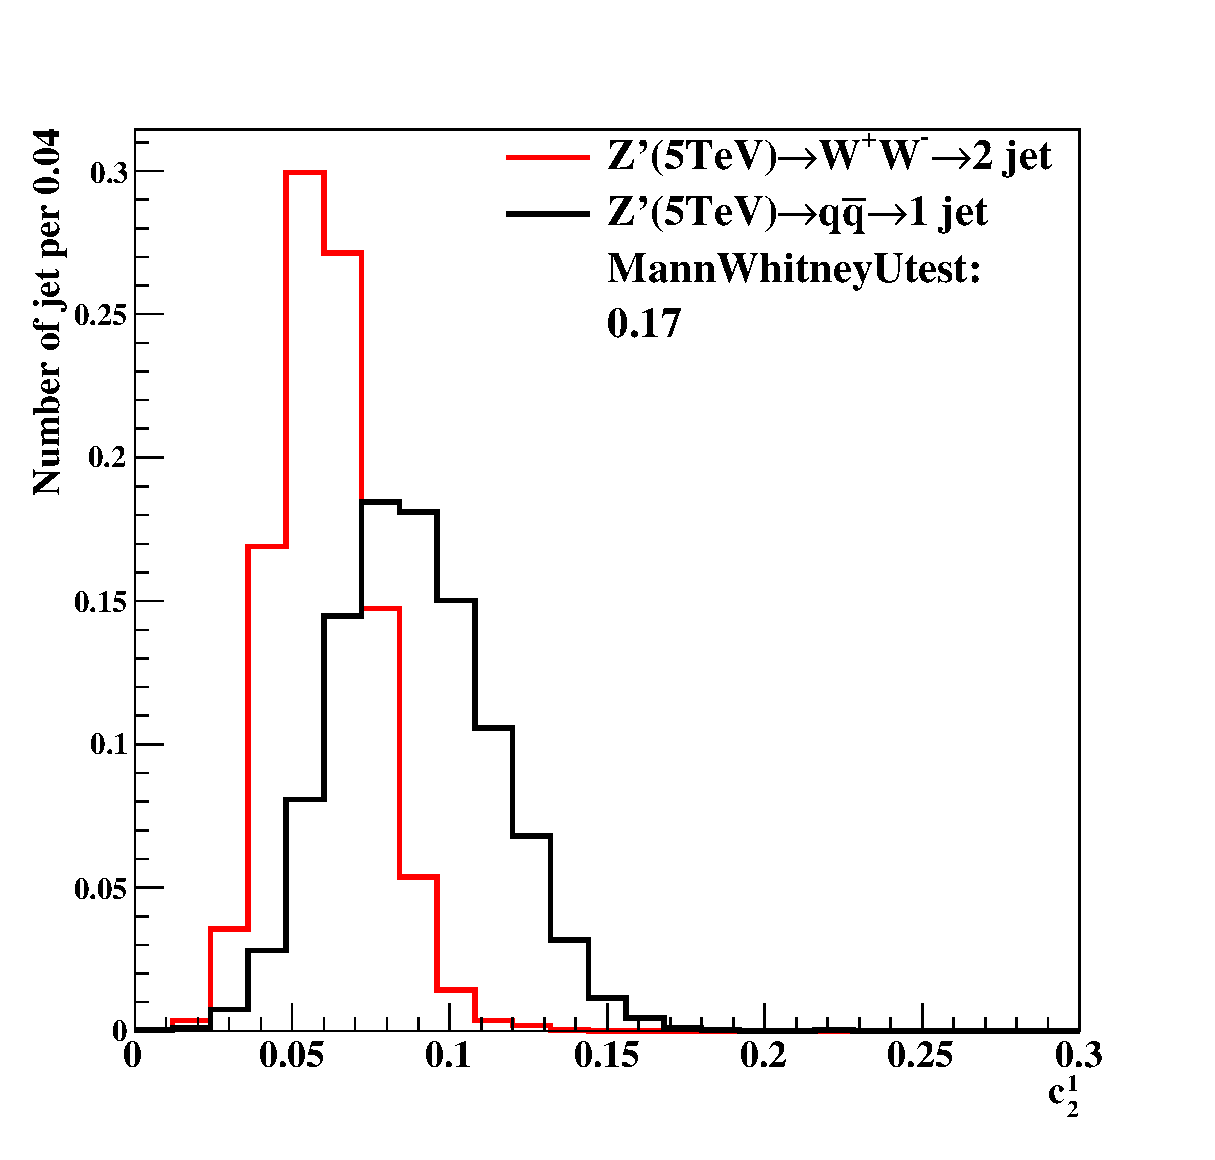
\includegraphics[width=0.43\textwidth]{figs/Dis_cluster_009_c2b1_5tev_04_Man.eps}
   }
   \subfigure[10TeV at 5$\times$5(cm$\times$cm) in cluster] {
   \includegraphics[width=0.43\textwidth]{figs/Dis_cluster_009_c2b1_10tev_04_Man.eps}
   }
   \subfigure[5TeV at 1$\times$1(cm$\times$cm) in cluster] {
   \includegraphics[width=0.43\textwidth]{figs/Dis_cluster_012_c2b1_5tev_04_Man.eps}
   }
   \subfigure[10TeV at 1$\times$1(cm$\times$cm) in cluster] {
   \includegraphics[width=0.43\textwidth]{figs/Dis_cluster_012_c2b1_10tev_04_Man.eps}
   }

\end{center}
\caption{Distributions of Mann-Whitney value U in 5,10TeV energy collision for $c_2^{(1)}$ in different detector sizes. Cell Size in 20$\times$20, 5$\times$5, and 1$\times$1(cm$\times$cm) are shown here.}
\label{fig:cluster_tau21_tau32}
\end{figure}

\begin{figure}
\begin{center}
   \subfigure[20TeV at 20$\times$20(cm$\times$cm) in cluster] {
   \includegraphics[width=0.43\textwidth]{figs/Dis_cluster_010_c2b1_20tev_04_Man.eps}\hfill
   }
   \subfigure[40TeV at 20$\times$20(cm$\times$cm) in cluster] {
   \includegraphics[width=0.43\textwidth]{figs/Dis_cluster_010_c2b1_40tev_04_Man.eps}
   }
   \subfigure[20TeV at 5$\times$5(cm$\times$cm) in cluster] {
   \includegraphics[width=0.43\textwidth]{figs/Dis_cluster_009_c2b1_20tev_04_Man.eps}
   }
   \subfigure[40TeV at 5$\times$5(cm$\times$cm) in cluster] {
   \includegraphics[width=0.43\textwidth]{figs/Dis_cluster_009_c2b1_40tev_04_Man.eps}
   }
   \subfigure[20TeV at 1$\times$1(cm$\times$cm) in cluster] {
   \includegraphics[width=0.43\textwidth]{figs/Dis_cluster_012_c2b1_20tev_04_Man.eps}
   }
   \subfigure[40TeV at 1$\times$1(cm$\times$cm) in cluster] {
   \includegraphics[width=0.43\textwidth]{figs/Dis_cluster_012_c2b1_40tev_04_Man.eps}
   }

\end{center}
\caption{Distributions of Mann-Whitney value U in 20,40TeV energy collision for $c_2^{(1)}$ in different detector sizes. Cell Size in 20$\times$20, 5$\times$5, and 1$\times$1(cm$\times$cm) are shown here.}
\label{fig:cluster_tau21_tau32}
\end{figure}

%25bins
\begin{figure}
\begin{center}
   \subfigure[5TeV at 20$\times$20(cm$\times$cm) in cluster] {
   \includegraphics[width=0.43\textwidth]{figs/Dis_cluster_010_tau21_5tev_04_Man.eps}\hfill
   }
   \subfigure[10TeV at 20$\times$20(cm$\times$cm) in cluster] {
   \includegraphics[width=0.43\textwidth]{figs/Dis_cluster_010_tau21_10tev_04_Man.eps}
   }
   \subfigure[5TeV at 5$\times$5(cm$\times$cm) in cluster] {
   \includegraphics[width=0.43\textwidth]{figs/Dis_cluster_009_tau21_5tev_04_Man.eps}
   }
   \subfigure[10TeV at 5$\times$5(cm$\times$cm) in cluster] {
   \includegraphics[width=0.43\textwidth]{figs/Dis_cluster_009_tau21_10tev_04_Man.eps}
   }
   \subfigure[5TeV at 1$\times$1(cm$\times$cm) in cluster] {
   \includegraphics[width=0.43\textwidth]{figs/Dis_cluster_012_tau21_5tev_04_Man.eps}
   }
   \subfigure[10TeV at 1$\times$1(cm$\times$cm) in cluster] {
   \includegraphics[width=0.43\textwidth]{figs/Dis_cluster_012_tau21_10tev_04_Man.eps}
   }

\end{center}
\caption{Distributions of Mann-Whitney value U in 5,10TeV energy collision for $\tau_{21}$ in different detector sizes. Cell Size in 20$\times$20, 5$\times$5, and 1$\times$1(cm$\times$cm) are shown here.}
\label{fig:cluster_tau21_tau32}
\end{figure}

\begin{figure}
\begin{center}
   \subfigure[20TeV at 20$\times$20(cm$\times$cm) in cluster] {
   \includegraphics[width=0.43\textwidth]{figs/Dis_cluster_010_tau21_20tev_04_Man.eps}\hfill
   }
   \subfigure[40TeV at 20$\times$20(cm$\times$cm) in cluster] {
   \includegraphics[width=0.43\textwidth]{figs/Dis_cluster_010_tau21_40tev_04_Man.eps}
   }
   \subfigure[20TeV at 5$\times$5(cm$\times$cm) in cluster] {
   \includegraphics[width=0.43\textwidth]{figs/Dis_cluster_009_tau21_20tev_04_Man.eps}
   }
   \subfigure[40TeV at 5$\times$5(cm$\times$cm) in cluster] {
   \includegraphics[width=0.43\textwidth]{figs/Dis_cluster_009_tau21_40tev_04_Man.eps}
   }
   \subfigure[20TeV at 1$\times$1(cm$\times$cm) in cluster] {
   \includegraphics[width=0.43\textwidth]{figs/Dis_cluster_012_tau21_20tev_04_Man.eps}
   }
   \subfigure[40TeV at 1$\times$1(cm$\times$cm) in cluster] {
   \includegraphics[width=0.43\textwidth]{figs/Dis_cluster_012_tau21_40tev_04_Man.eps}
   }

\end{center}
\caption{Distributions of Mann-Whitney value U in 20,40TeV energy collision for $\tau_{21}$ in different detector sizes. Cell Size in 20$\times$20, 5$\times$5, and 1$\times$1(cm$\times$cm) are shown here.}
\label{fig:cluster_tau21_tau32}
\end{figure}

%25bins
\begin{figure}
\begin{center}
   \subfigure[5TeV at 20$\times$20(cm$\times$cm) in cluster] {
   \includegraphics[width=0.43\textwidth]{figs/Dis_cluster_010_tau32_5tev_04_Man.eps}\hfill
   }
   \subfigure[10TeV at 20$\times$20(cm$\times$cm) in cluster] {
   \includegraphics[width=0.43\textwidth]{figs/Dis_cluster_010_tau32_10tev_04_Man.eps}
   }
   \subfigure[5TeV at 5$\times$5(cm$\times$cm) in cluster] {
   \includegraphics[width=0.43\textwidth]{figs/Dis_cluster_009_tau32_5tev_04_Man.eps}
   }
   \subfigure[10TeV at 5$\times$5(cm$\times$cm) in cluster] {
   \includegraphics[width=0.43\textwidth]{figs/Dis_cluster_009_tau32_10tev_04_Man.eps}
   }
   \subfigure[5TeV at 1$\times$1(cm$\times$cm) in cluster] {
   \includegraphics[width=0.43\textwidth]{figs/Dis_cluster_012_tau32_5tev_04_Man.eps}
   }
   \subfigure[10TeV at 1$\times$1(cm$\times$cm) in cluster] {
   \includegraphics[width=0.43\textwidth]{figs/Dis_cluster_012_tau32_10tev_04_Man.eps}
   }

\end{center}
\caption{Distributions of Mann-Whitney value U in 5,10TeV energy collision for $\tau_{32}$ in different detector sizes. Cell Size in 20$\times$20, 5$\times$5, and 1$\times$1(cm$\times$cm) are shown here.}
\label{fig:cluster_tau21_tau32}
\end{figure}

\begin{figure}
\begin{center}
   \subfigure[20TeV at 20$\times$20(cm$\times$cm) in cluster] {
   \includegraphics[width=0.43\textwidth]{figs/Dis_cluster_010_tau32_20tev_04_Man.eps}\hfill
   }
   \subfigure[40TeV at 20$\times$20(cm$\times$cm) in cluster] {
   \includegraphics[width=0.43\textwidth]{figs/Dis_cluster_010_tau32_40tev_04_Man.eps}
   }
   \subfigure[20TeV at 5$\times$5(cm$\times$cm) in cluster] {
   \includegraphics[width=0.43\textwidth]{figs/Dis_cluster_009_tau32_20tev_04_Man.eps}
   }
   \subfigure[40TeV at 5$\times$5(cm$\times$cm) in cluster] {
   \includegraphics[width=0.43\textwidth]{figs/Dis_cluster_009_tau32_40tev_04_Man.eps}
   }
   \subfigure[20TeV at 1$\times$1(cm$\times$cm) in cluster] {
   \includegraphics[width=0.43\textwidth]{figs/Dis_cluster_012_tau32_20tev_04_Man.eps}
   }
   \subfigure[40TeV at 1$\times$1(cm$\times$cm) in cluster] {
   \includegraphics[width=0.43\textwidth]{figs/Dis_cluster_012_tau32_40tev_04_Man.eps}
   }

\end{center}
\caption{Distributions of Mann-Whitney value U in 20,40TeV energy collision for $\tau_{32}$ in different detector sizes. Cell Size in 20$\times$20, 5$\times$5, and 1$\times$1(cm$\times$cm) are shown here.}
\label{fig:cluster_tau21_tau32}
\end{figure}

%25bins
\begin{figure}
\begin{center}
   \subfigure[5TeV at 20$\times$20(cm$\times$cm) cut at 0.5GeV] {
   \includegraphics[width=0.43\textwidth]{figs/Dis_Rawhit_05GeV_010_c2b1_5tev_04_Man.eps}\hfill
   }
   \subfigure[10TeV at 20$\times$20(cm$\times$cm) cut at 0.5GeV] {
   \includegraphics[width=0.43\textwidth]{figs/Dis_Rawhit_05GeV_010_c2b1_10tev_04_Man.eps}
   }
   \subfigure[5TeV at 5$\times$5(cm$\times$cm) cut at 0.5GeV] {
   \includegraphics[width=0.43\textwidth]{figs/Dis_Rawhit_05GeV_009_c2b1_5tev_04_Man.eps}
   }
   \subfigure[10TeV at 5$\times$5(cm$\times$cm) cut at 0.5GeV] {
   \includegraphics[width=0.43\textwidth]{figs/Dis_Rawhit_05GeV_009_c2b1_10tev_04_Man.eps}
   }
   \subfigure[5TeV at 1$\times$1(cm$\times$cm) cut at 0.5GeV] {
   \includegraphics[width=0.43\textwidth]{figs/Dis_Rawhit_05GeV_012_c2b1_5tev_04_Man.eps}
   }
   \subfigure[10TeV at 1$\times$1(cm$\times$cm) cut at 0.5GeV] {
   \includegraphics[width=0.43\textwidth]{figs/Dis_Rawhit_05GeV_012_c2b1_10tev_04_Man.eps}
   }

\end{center}
\caption{Distributions of Mann-Whitney value U in 5,10TeV energy collision for $c_2^{(1)}$ in different detector sizes. Cell Size in 20$\times$20, 5$\times$5, and 1$\times$1(cm$\times$cm) are shown here.}
\label{fig:cluster_tau21_tau32}
\end{figure}

\begin{figure}
\begin{center}
   \subfigure[20TeV at 20$\times$20(cm$\times$cm) cut at 0.5GeV] {
   \includegraphics[width=0.43\textwidth]{figs/Dis_Rawhit_05GeV_010_c2b1_20tev_04_Man.eps}\hfill
   }
   \subfigure[40TeV at 20$\times$20(cm$\times$cm) cut at 0.5GeV] {
   \includegraphics[width=0.43\textwidth]{figs/Dis_Rawhit_05GeV_010_c2b1_40tev_04_Man.eps}
   }
   \subfigure[20TeV at 5$\times$5(cm$\times$cm) cut at 0.5GeV] {
   \includegraphics[width=0.43\textwidth]{figs/Dis_Rawhit_05GeV_009_c2b1_20tev_04_Man.eps}
   }
   \subfigure[40TeV at 5$\times$5(cm$\times$cm) cut at 0.5GeV] {
   \includegraphics[width=0.43\textwidth]{figs/Dis_Rawhit_05GeV_009_c2b1_40tev_04_Man.eps}
   }
   \subfigure[20TeV at 1$\times$1(cm$\times$cm) cut at 0.5GeV] {
   \includegraphics[width=0.43\textwidth]{figs/Dis_Rawhit_05GeV_012_c2b1_20tev_04_Man.eps}
   }
   \subfigure[40TeV at 1$\times$1(cm$\times$cm) cut at 0.5GeV] {
   \includegraphics[width=0.43\textwidth]{figs/Dis_Rawhit_05GeV_012_c2b1_40tev_04_Man.eps}
   }

\end{center}
\caption{Distributions of Mann-Whitney value U in 20,40TeV energy collision for $c_2^{(1)}$ in different detector sizes. Cell Size in 20$\times$20, 5$\times$5, and 1$\times$1(cm$\times$cm) are shown here.}
\label{fig:cluster_tau21_tau32}
\end{figure}

%25bins
\begin{figure}
\begin{center}
   \subfigure[5TeV at 20$\times$20(cm$\times$cm) cut at 0.5GeV] {
   \includegraphics[width=0.43\textwidth]{figs/Dis_Rawhit_05GeV_010_tau21_5tev_04_Man.eps}\hfill
   }
   \subfigure[10TeV at 20$\times$20(cm$\times$cm) cut at 0.5GeV] {
   \includegraphics[width=0.43\textwidth]{figs/Dis_Rawhit_05GeV_010_tau21_10tev_04_Man.eps}
   }
   \subfigure[5TeV at 5$\times$5(cm$\times$cm) cut at 0.5GeV] {
   \includegraphics[width=0.43\textwidth]{figs/Dis_Rawhit_05GeV_009_tau21_5tev_04_Man.eps}
   }
   \subfigure[10TeV at 5$\times$5(cm$\times$cm) cut at 0.5GeV] {
   \includegraphics[width=0.43\textwidth]{figs/Dis_Rawhit_05GeV_009_tau21_10tev_04_Man.eps}
   }
   \subfigure[5TeV at 1$\times$1(cm$\times$cm) cut at 0.5GeV] {
   \includegraphics[width=0.43\textwidth]{figs/Dis_Rawhit_05GeV_012_tau21_5tev_04_Man.eps}
   }
   \subfigure[10TeV at 1$\times$1(cm$\times$cm) cut at 0.5GeV] {
   \includegraphics[width=0.43\textwidth]{figs/Dis_Rawhit_05GeV_012_tau21_10tev_04_Man.eps}
   }

\end{center}
\caption{Distributions of Mann-Whitney value U in 5,10TeV energy collision for $\tau_{21}$ in different detector sizes. Cell Size in 20$\times$20, 5$\times$5, and 1$\times$1(cm$\times$cm) are shown here.}
\label{fig:cluster_tau21_tau32}
\end{figure}

\begin{figure}
\begin{center}
   \subfigure[20TeV at 20$\times$20(cm$\times$cm) cut at 0.5GeV] {
   \includegraphics[width=0.43\textwidth]{figs/Dis_Rawhit_05GeV_010_tau21_20tev_04_Man.eps}\hfill
   }
   \subfigure[40TeV at 20$\times$20(cm$\times$cm) cut at 0.5GeV] {
   \includegraphics[width=0.43\textwidth]{figs/Dis_Rawhit_05GeV_010_tau21_40tev_04_Man.eps}
   }
   \subfigure[20TeV at 5$\times$5(cm$\times$cm) cut at 0.5GeV] {
   \includegraphics[width=0.43\textwidth]{figs/Dis_Rawhit_05GeV_009_tau21_20tev_04_Man.eps}
   }
   \subfigure[40TeV at 5$\times$5(cm$\times$cm) icut at 0.5GeV] {
   \includegraphics[width=0.43\textwidth]{figs/Dis_Rawhit_05GeV_009_tau21_40tev_04_Man.eps}
   }
   \subfigure[20TeV at 1$\times$1(cm$\times$cm) cut at 0.5GeV] {
   \includegraphics[width=0.43\textwidth]{figs/Dis_Rawhit_05GeV_012_tau21_20tev_04_Man.eps}
   }
   \subfigure[40TeV at 1$\times$1(cm$\times$cm) cut at 0.5GeV] {
   \includegraphics[width=0.43\textwidth]{figs/Dis_Rawhit_05GeV_012_tau21_40tev_04_Man.eps}
   }

\end{center}
\caption{Distributions of Mann-Whitney value U in 20,40TeV energy collision for $\tau_{21}$ in different detector sizes. Cell Size in 20$\times$20, 5$\times$5, and 1$\times$1(cm$\times$cm) are shown here.}
\label{fig:cluster_tau21_tau32}
\end{figure}

%25bins
\begin{figure}
\begin{center}
   \subfigure[5TeV at 20$\times$20(cm$\times$cm) cut at 0.5GeV] {
   \includegraphics[width=0.43\textwidth]{figs/Dis_Rawhit_05GeV_010_tau32_5tev_04_Man.eps}\hfill
   }
   \subfigure[10TeV at 20$\times$20(cm$\times$cm) cut at 0.5GeV] {
   \includegraphics[width=0.43\textwidth]{figs/Dis_Rawhit_05GeV_010_tau32_10tev_04_Man.eps}
   }
   \subfigure[5TeV at 5$\times$5(cm$\times$cm) cut at 0.5GeV] {
   \includegraphics[width=0.43\textwidth]{figs/Dis_Rawhit_05GeV_009_tau32_5tev_04_Man.eps}
   }
   \subfigure[10TeV at 5$\times$5(cm$\times$cm) cut at 0.5GeV] {
   \includegraphics[width=0.43\textwidth]{figs/Dis_Rawhit_05GeV_009_tau32_10tev_04_Man.eps}
   }
   \subfigure[5TeV at 1$\times$1(cm$\times$cm) cut at 0.5GeV] {
   \includegraphics[width=0.43\textwidth]{figs/Dis_Rawhit_05GeV_012_tau32_5tev_04_Man.eps}
   }
   \subfigure[10TeV at 1$\times$1(cm$\times$cm) cut at 0.5GeV] {
   \includegraphics[width=0.43\textwidth]{figs/Dis_Rawhit_05GeV_012_tau32_10tev_04_Man.eps}
   }

\end{center}
\caption{Distributions of Mann-Whitney value U in 5,10TeV energy collision for $\tau_{32}$ in different detector sizes. Cell Size in 20$\times$20, 5$\times$5, and 1$\times$1(cm$\times$cm) are shown here.}
\label{fig:cluster_tau21_tau32}
\end{figure}

\begin{figure}
\begin{center}
   \subfigure[20TeV at 20$\times$20(cm$\times$cm) cut at 0.5GeV] {
   \includegraphics[width=0.43\textwidth]{figs/Dis_Rawhit_05GeV_010_tau32_20tev_04_Man.eps}\hfill
   }
   \subfigure[40TeV at 20$\times$20(cm$\times$cm) cut at 0.5GeV] {
   \includegraphics[width=0.43\textwidth]{figs/Dis_Rawhit_05GeV_010_tau32_40tev_04_Man.eps}
   }
   \subfigure[20TeV at 5$\times$5(cm$\times$cm) cut at 0.5GeV] {
   \includegraphics[width=0.43\textwidth]{figs/Dis_Rawhit_05GeV_009_tau32_20tev_04_Man.eps}
   }
   \subfigure[40TeV at 5$\times$5(cm$\times$cm) cut at 0.5GeV] {
   \includegraphics[width=0.43\textwidth]{figs/Dis_Rawhit_05GeV_009_tau32_40tev_04_Man.eps}
   }
   \subfigure[20TeV at 1$\times$1(cm$\times$cm) cut at 0.5GeV] {
   \includegraphics[width=0.43\textwidth]{figs/Dis_Rawhit_05GeV_012_tau32_20tev_04_Man.eps}
   }
   \subfigure[40TeV at 1$\times$1(cm$\times$cm) cut at 0.5GeV] {
   \includegraphics[width=0.43\textwidth]{figs/Dis_Rawhit_05GeV_012_tau32_40tev_04_Man.eps}
   }

\end{center}
\caption{Distributions of Mann-Whitney value U in 20,40TeV energy collision for $\tau_{32}$ in different detector sizes. Cell Size in 20$\times$20, 5$\times$5, and 1$\times$1(cm$\times$cm) are shown here.}
\label{fig:cluster_tau21_tau32}
\end{figure}

%25bins
\begin{figure}
\begin{center}
   \subfigure[5TeV at 20$\times$20(cm$\times$cm) cut at 0.25GeV] {
   \includegraphics[width=0.43\textwidth]{figs/Dis_Rawhit_025GeV_010_c2b1_5tev_04_Man.eps}\hfill
   }
   \subfigure[10TeV at 20$\times$20(cm$\times$cm) cut at 0.25GeV] {
   \includegraphics[width=0.43\textwidth]{figs/Dis_Rawhit_025GeV_010_c2b1_10tev_04_Man.eps}
   }
   \subfigure[5TeV at 5$\times$5(cm$\times$cm) cut at 0.25GeV] {
   \includegraphics[width=0.43\textwidth]{figs/Dis_Rawhit_025GeV_009_c2b1_5tev_04_Man.eps}
   }
   \subfigure[10TeV at 5$\times$5(cm$\times$cm) cut at 0.25GeV] {
   \includegraphics[width=0.43\textwidth]{figs/Dis_Rawhit_025GeV_009_c2b1_10tev_04_Man.eps}
   }
   \subfigure[5TeV at 1$\times$1(cm$\times$cm) cut at 0.25GeV] {
   \includegraphics[width=0.43\textwidth]{figs/Dis_Rawhit_025GeV_012_c2b1_5tev_04_Man.eps}
   }
   \subfigure[10TeV at 1$\times$1(cm$\times$cm) cut at 0.25GeV] {
   \includegraphics[width=0.43\textwidth]{figs/Dis_Rawhit_025GeV_012_c2b1_10tev_04_Man.eps}
   }

\end{center}
\caption{Distributions of Mann-Whitney value U in 5,10TeV energy collision for $c_2^{(1)}$ in different detector sizes. Cell Size in 20$\times$20, 5$\times$5, and 1$\times$1(cm$\times$cm) are shown here.}
\label{fig:cluster_tau21_tau32}
\end{figure}

\begin{figure}
\begin{center}
   \subfigure[20TeV at 20$\times$20(cm$\times$cm) cut at 0.25GeV] {
   \includegraphics[width=0.43\textwidth]{figs/Dis_Rawhit_025GeV_010_c2b1_20tev_04_Man.eps}\hfill
   }
   \subfigure[40TeV at 20$\times$20(cm$\times$cm) cut at 0.25GeV] {
   \includegraphics[width=0.43\textwidth]{figs/Dis_Rawhit_025GeV_010_c2b1_40tev_04_Man.eps}
   }
   \subfigure[20TeV at 5$\times$5(cm$\times$cm) cut at 0.25GeV] {
   \includegraphics[width=0.43\textwidth]{figs/Dis_Rawhit_025GeV_009_c2b1_20tev_04_Man.eps}
   }
   \subfigure[40TeV at 5$\times$5(cm$\times$cm) cut at 0.25GeV] {
   \includegraphics[width=0.43\textwidth]{figs/Dis_Rawhit_025GeV_009_c2b1_40tev_04_Man.eps}
   }
   \subfigure[20TeV at 1$\times$1(cm$\times$cm) cut at 0.25GeV] {
   \includegraphics[width=0.43\textwidth]{figs/Dis_Rawhit_025GeV_012_c2b1_20tev_04_Man.eps}
   }
   \subfigure[40TeV at 1$\times$1(cm$\times$cm) cut at 0.25GeV] {
   \includegraphics[width=0.43\textwidth]{figs/Dis_Rawhit_025GeV_012_c2b1_40tev_04_Man.eps}
   }

\end{center}
\caption{Distributions of Mann-Whitney value U in 20,40TeV energy collision for $c_2^{(1)}$ in different detector sizes. Cell Size in 20$\times$20, 5$\times$5, and 1$\times$1(cm$\times$cm) are shown here.}
\label{fig:cluster_tau21_tau32}
\end{figure}

%25bins
\begin{figure}
\begin{center}
   \subfigure[5TeV at 20$\times$20(cm$\times$cm) cut at 0.25GeV] {
   \includegraphics[width=0.43\textwidth]{figs/Dis_Rawhit_025GeV_010_tau21_5tev_04_Man.eps}\hfill
   }
   \subfigure[10TeV at 20$\times$20(cm$\times$cm) cut at 0.25GeV] {
   \includegraphics[width=0.43\textwidth]{figs/Dis_Rawhit_025GeV_010_tau21_10tev_04_Man.eps}
   }
   \subfigure[5TeV at 5$\times$5(cm$\times$cm) cut at 0.25GeV] {
   \includegraphics[width=0.43\textwidth]{figs/Dis_Rawhit_025GeV_009_tau21_5tev_04_Man.eps}
   }
   \subfigure[10TeV at 5$\times$5(cm$\times$cm) cut at 0.25GeV] {
   \includegraphics[width=0.43\textwidth]{figs/Dis_Rawhit_025GeV_009_tau21_10tev_04_Man.eps}
   }
   \subfigure[5TeV at 1$\times$1(cm$\times$cm) cut at 0.25GeV] {
   \includegraphics[width=0.43\textwidth]{figs/Dis_Rawhit_025GeV_012_tau21_5tev_04_Man.eps}
   }
   \subfigure[10TeV at 1$\times$1(cm$\times$cm) cut at 0.25GeV] {
   \includegraphics[width=0.43\textwidth]{figs/Dis_Rawhit_025GeV_012_tau21_10tev_04_Man.eps}
   }

\end{center}
\caption{Distributions of Mann-Whitney value U in 5,10TeV energy collision for $\tau_{21}$ in different detector sizes. Cell Size in 20$\times$20, 5$\times$5, and 1$\times$1(cm$\times$cm) are shown here.}
\label{fig:cluster_tau21_tau32}
\end{figure}

\begin{figure}
\begin{center}
   \subfigure[20TeV at 20$\times$20(cm$\times$cm) cut at 0.25GeV] {
   \includegraphics[width=0.43\textwidth]{figs/Dis_Rawhit_025GeV_010_tau21_20tev_04_Man.eps}\hfill
   }
   \subfigure[40TeV at 20$\times$20(cm$\times$cm) cut at 0.25GeV] {
   \includegraphics[width=0.43\textwidth]{figs/Dis_Rawhit_025GeV_010_tau21_40tev_04_Man.eps}
   }
   \subfigure[20TeV at 5$\times$5(cm$\times$cm) cut at 0.25GeV] {
   \includegraphics[width=0.43\textwidth]{figs/Dis_Rawhit_025GeV_009_tau21_20tev_04_Man.eps}
   }
   \subfigure[40TeV at 5$\times$5(cm$\times$cm) icut at 0.25GeV] {
   \includegraphics[width=0.43\textwidth]{figs/Dis_Rawhit_025GeV_009_tau21_40tev_04_Man.eps}
   }
   \subfigure[20TeV at 1$\times$1(cm$\times$cm) cut at 0.25GeV] {
   \includegraphics[width=0.43\textwidth]{figs/Dis_Rawhit_025GeV_012_tau21_20tev_04_Man.eps}
   }
   \subfigure[40TeV at 1$\times$1(cm$\times$cm) cut at 0.25GeV] {
   \includegraphics[width=0.43\textwidth]{figs/Dis_Rawhit_025GeV_012_tau21_40tev_04_Man.eps}
   }

\end{center}
\caption{Distributions of Mann-Whitney value U in 20,40TeV energy collision for $\tau_{21}$ in different detector sizes. Cell Size in 20$\times$20, 5$\times$5, and 1$\times$1(cm$\times$cm) are shown here.}
\label{fig:cluster_tau21_tau32}
\end{figure}

%25bins
\begin{figure}
\begin{center}
   \subfigure[5TeV at 20$\times$20(cm$\times$cm) cut at 0.25GeV] {
   \includegraphics[width=0.43\textwidth]{figs/Dis_Rawhit_025GeV_010_tau32_5tev_04_Man.eps}\hfill
   }
   \subfigure[10TeV at 20$\times$20(cm$\times$cm) cut at 0.25GeV] {
   \includegraphics[width=0.43\textwidth]{figs/Dis_Rawhit_025GeV_010_tau32_10tev_04_Man.eps}
   }
   \subfigure[5TeV at 5$\times$5(cm$\times$cm) cut at 0.25GeV] {
   \includegraphics[width=0.43\textwidth]{figs/Dis_Rawhit_025GeV_009_tau32_5tev_04_Man.eps}
   }
   \subfigure[10TeV at 5$\times$5(cm$\times$cm) cut at 0.25GeV] {
   \includegraphics[width=0.43\textwidth]{figs/Dis_Rawhit_025GeV_009_tau32_10tev_04_Man.eps}
   }
   \subfigure[5TeV at 1$\times$1(cm$\times$cm) cut at 0.25GeV] {
   \includegraphics[width=0.43\textwidth]{figs/Dis_Rawhit_025GeV_012_tau32_5tev_04_Man.eps}
   }
   \subfigure[10TeV at 1$\times$1(cm$\times$cm) cut at 0.25GeV] {
   \includegraphics[width=0.43\textwidth]{figs/Dis_Rawhit_025GeV_012_tau32_10tev_04_Man.eps}
   }

\end{center}
\caption{Distributions of Mann-Whitney value U in 5,10TeV energy collision for $\tau_{32}$ in different detector sizes. Cell Size in 20$\times$20, 5$\times$5, and 1$\times$1(cm$\times$cm) are shown here.}
\label{fig:cluster_tau21_tau32}
\end{figure}

\begin{figure}
\begin{center}
   \subfigure[20TeV at 20$\times$20(cm$\times$cm) cut at 0.25GeV] {
   \includegraphics[width=0.43\textwidth]{figs/Dis_Rawhit_025GeV_010_tau32_20tev_04_Man.eps}\hfill
   }
   \subfigure[40TeV at 20$\times$20(cm$\times$cm) cut at 0.25GeV] {
   \includegraphics[width=0.43\textwidth]{figs/Dis_Rawhit_025GeV_010_tau32_40tev_04_Man.eps}
   }
   \subfigure[20TeV at 5$\times$5(cm$\times$cm) cut at 0.25GeV] {
   \includegraphics[width=0.43\textwidth]{figs/Dis_Rawhit_025GeV_009_tau32_20tev_04_Man.eps}
   }
   \subfigure[40TeV at 5$\times$5(cm$\times$cm) cut at 0.25GeV] {
   \includegraphics[width=0.43\textwidth]{figs/Dis_Rawhit_025GeV_009_tau32_40tev_04_Man.eps}
   }
   \subfigure[20TeV at 1$\times$1(cm$\times$cm) cut at 0.25GeV] {
   \includegraphics[width=0.43\textwidth]{figs/Dis_Rawhit_025GeV_012_tau32_20tev_04_Man.eps}
   }
   \subfigure[40TeV at 1$\times$1(cm$\times$cm) cut at 0.25GeV] {
   \includegraphics[width=0.43\textwidth]{figs/Dis_Rawhit_025GeV_012_tau32_40tev_04_Man.eps}
   }

\end{center}
\caption{Distributions of Mann-Whitney value U in 20,40TeV energy collision for $\tau_{32}$ in different detector sizes. Cell Size in 20$\times$20, 5$\times$5, and 1$\times$1(cm$\times$cm) are shown here.}
\label{fig:cluster_tau21_tau32}
\end{figure}

%25bins
\begin{figure}
\begin{center}
   \subfigure[$\tau_{21}$ in cluster] {
   \includegraphics[width=0.43\textwidth]{figs/cluster_tau21_summary_U.eps}\hfill
   }
   \subfigure[$\tau_{32}$ in cluster] {
   \includegraphics[width=0.43\textwidth]{figs/cluster_tau32_summary_U.eps}
   }
   \subfigure[$c_2^{(1)}$ in cluster] {
   \includegraphics[width=0.43\textwidth]{figs/cluster_c2b1_summary_U.eps}
   }
\end{center}
\caption{The Mann-Whitney U values for $\tau_{21}$,$\tau_{32}$ and $c_2^{(1)}$ reconstructed from calorimeter clusters at different collision energies correspond to different detector sizes in cluster. The energies of collision at 5, 10, 20, 40TeV are shown in each figure.}
\label{fig:cluster_U_summary}
\end{figure}


%25bins
\begin{figure}
\begin{center}
   \subfigure[$\tau_{21}$ rawhit cut at 0.5GeV] {
   \includegraphics[width=0.43\textwidth]{figs/Rawhit_05GeV_tau21_summary_U.eps}\hfill
   }
   \subfigure[$\tau_{32}$ rawhit cut at 0.5GeV] {
   \includegraphics[width=0.43\textwidth]{figs/Rawhit_05GeV_tau32_summary_U.eps}
   }
   \subfigure[$c_2^{(1)}$ rawhit cut at 0.5GeV] {
   \includegraphics[width=0.43\textwidth]{figs/Rawhit_05GeV_c2b1_summary_U.eps}
   }
\end{center}
\caption{The Mann-Whitney U values for $\tau_{21}$,$\tau_{32}$ and $c_2^{(1)}$ reconstructed from calorimeter hit at 05GeV cut at different collision energies correspond to different detector sizes in rawhit cut at 05GeV. The energies of collision at 5, 10, 20, 40TeV are shown in each figure.}
\label{fig:raw_U_summary}
\end{figure}

%25bins
\begin{figure}
\begin{center}
   \subfigure[$\tau_{21}$ rawhit cut at 0.25GeV] {
   \includegraphics[width=0.43\textwidth]{figs/Rawhit_025GeV_tau21_summary_U.eps}\hfill
   }
   \subfigure[$\tau_{32}$ rawhit cut at 0.25GeV] {
   \includegraphics[width=0.43\textwidth]{figs/Rawhit_025GeV_tau32_summary_U.eps}
   }
   \subfigure[$c_2^{(1)}$ rawhit cut at 0.25GeV] {
   \includegraphics[width=0.43\textwidth]{figs/Rawhit_025GeV_c2b1_summary_U.eps}
   }
\end{center}
\caption{The Mann-Whitney U values for $\tau_{21}$,$\tau_{32}$ and $c_2^{(1)}$ reconstructed from calorimeter hit at 0.25GeV cut at different collision energies correspond to different detector sizes in cluster. The energies of collision at 5, 10, 20, 40TeV are shown in each figure.}
\label{fig:cluster_U_summary}
\end{figure}
\end{document}



